
\chapter{Muminav}

Beispiel Progamm, welches zeigt wie man Muminav einbinden kann.

relevante andere Projekte - hoch spezifizierte Anforderungen

\section{Lizenz}

Vorgabe war, die gesamte Entwicklungsarbeit als Open Source
Projekt durchzuf�hren. Dies schlie�t ein, die
Projektergebnisse unter einer Open Source Lizenz \cite{OSI2002} zu ver�ffentlichen.\\
Da wir unser Projekt in Zusammenarbeit mit der Mumie-Gruppe
entwickeln, mussten wir uns im Vorfeld mit Ihnen auf eine Open
Source Lizenz verst�ndigen, welche in das Gesamtprojekt
\textsc{Mumie}
integrierbar ist.\\
Die GPL \cite{GPL1991} (GNU General Public License)



LGPL \cite{LGPL1999}.

\section{Entwicklungsumgebung}
\subsection{Enwicklungswerkzeuge}
F�r das Projekt wurden eine Reihe von Entwicklungswerkzeugen und
Technologien verwandt, welche f�r Open-Source-Projekte
charakteristisch sind:

\begin{itemize}

\item \textbf{Mailinglisten} um mit den Entwicklern und allen, die
sonst noch Interesse an dem Projekt haben zu kommunizieren. Wobei
damit auch gleichzeitig eine Dokumentation des Projektverlaufs
�ber die Maininglisten-Archive entsteht.
\item \textbf{CVS} Concurrent Version System \cite{FOGEL2000}.
Hat uns erm�glicht dezentral an den selben Quelldateien zu
arbeiten. �ber die CVS-Log Eintr�ge l�sst sich auch nachtr�glich
die Entwicklungs-Historie nachvollziehen.
\item \textbf{eMail} Als standard-Medium zum direkten pers�nlichen
Infromationsaustausch.
\item \textbf{Instant-Messageing} hat bei Arbeiten, die ein hohes
Ma� an Absprachen bed�rfen, nicht die Nachteile, die ein
asynchrones Medium wie eMail und Mailinglisten haben.
\item \textbf{Projekt-Homepage} Unter der URL:
\verb|http://muminav.berlios.de| haben wir eine Projekt-Homepage
angelegt, die, die �ffentlichkeit und die Teilnehmer des Projekts
mit allgemeinen Informationen versorgt.
\item \textbf{Newsgroups} Hier haben wir uns Anregungen und
Informationen f�r die Planung des Projekts und bei Problemen, die
in der t�glichen Arbeite aufraten besorgt.

%\item \textbf{}
\end{itemize}



F�r die Entwicklung der Quellen habe wir folgende Software
eingesetzt.

\begin{itemize}

\item \textbf{Java\trademark 2 Platform, Standard Edition}
\item \textbf{Apache Ant} des \textsc{Jakarta Projekt} von Apache,
als make-Tool.
\end{itemize}

Leider ist der Javacompiler, den wir eingesetzt haben nicht als
Open-Source ver�ffentlicht worden. Aus Kompatibilit�sgr�nden
mussten wir uns jedoch f�r diesen Compiler entscheiden, damit das
Applet unter m�glichst unterschiedlichen Umgebungen l�uft ohne,
dass der Benutzer weitere Software installieren muss.

Als Alternativen zum Java-Compiler von Sun w�re im
Open-Source-Bereich z.\,B\ \textsc{Jikes} von IBM \cite{JIKES},
der an der Univerist�t von Bosten entwicklete \textsc{Espresso}
\cite{ESPR} oder der \textsc{GCJ} der \textsc{Free Software
Foundation} \cite{GJC}, denkbar. Da sich aber jeder bei uns die
Java Quellcodes herunterladen kann, bleibt es jedem selbst
�berlassen, welchen Kompiler er einsetzt \cite{J2SE} .

\subsection{Projekthoster}

Bei der Wahl des Projekthosters kam f�r uns \textsc{SourceForge}
\emph{nicht} in Frage, da sich im Laufe der Zeit die
Lizenz-Politik \cite{SFORGE} des Hosters immer mehr gegen die
Ideale der Open-Source-Gemeinde richten. Das Savannah Projket der
Free Software Foundation war zu Projektbeginn leider noch nicht
gen�gend weit entwickelt.

Aus diesen Gr�nden haben wir uns f�r den Berliner Projekthoster
\textsc{Berlios} \cite{BerliOS} entschieden, der uns mit den
meisten Diensten unterst�tzen konnte.

\subsection{Probleme und ihre L�sungen}

XML-Parser mitliefern - Gr��e - Entscheidung f�r Java 1.4 und
Mozilla

\section{Verwendete Komponenten und Ressourcen}

\begin{figure}[htbp]
    \centering%
%   \setcapwidth[c]{12cm}%
    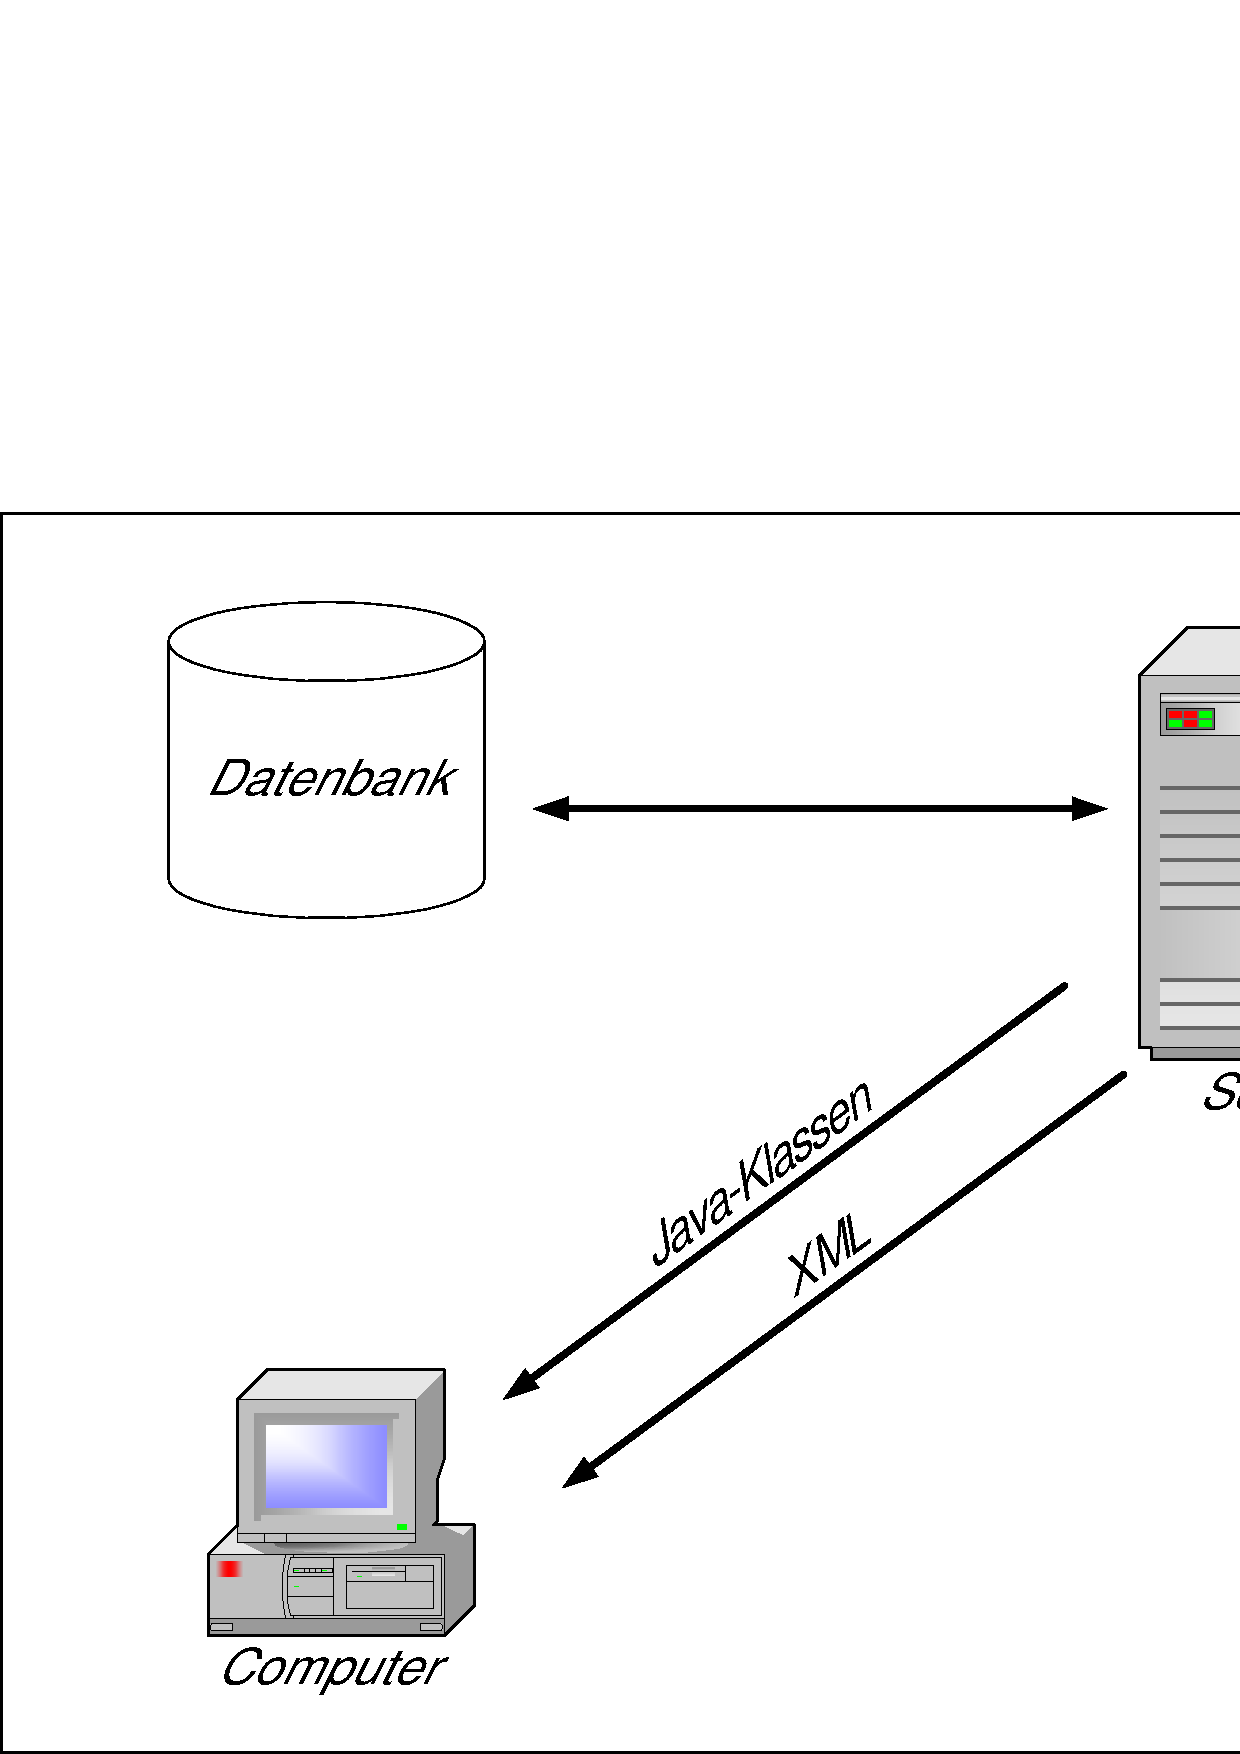
\includegraphics[width=10cm]{figs/kommunikation}
    \captionbelow{Kommunikation: Informationsfluss}
    \label{FIG:kommunikationsfluss}
\end{figure}

\begin{figure}[htbp]
    \centering%
%   \setcapwidth[c]{12cm}%
    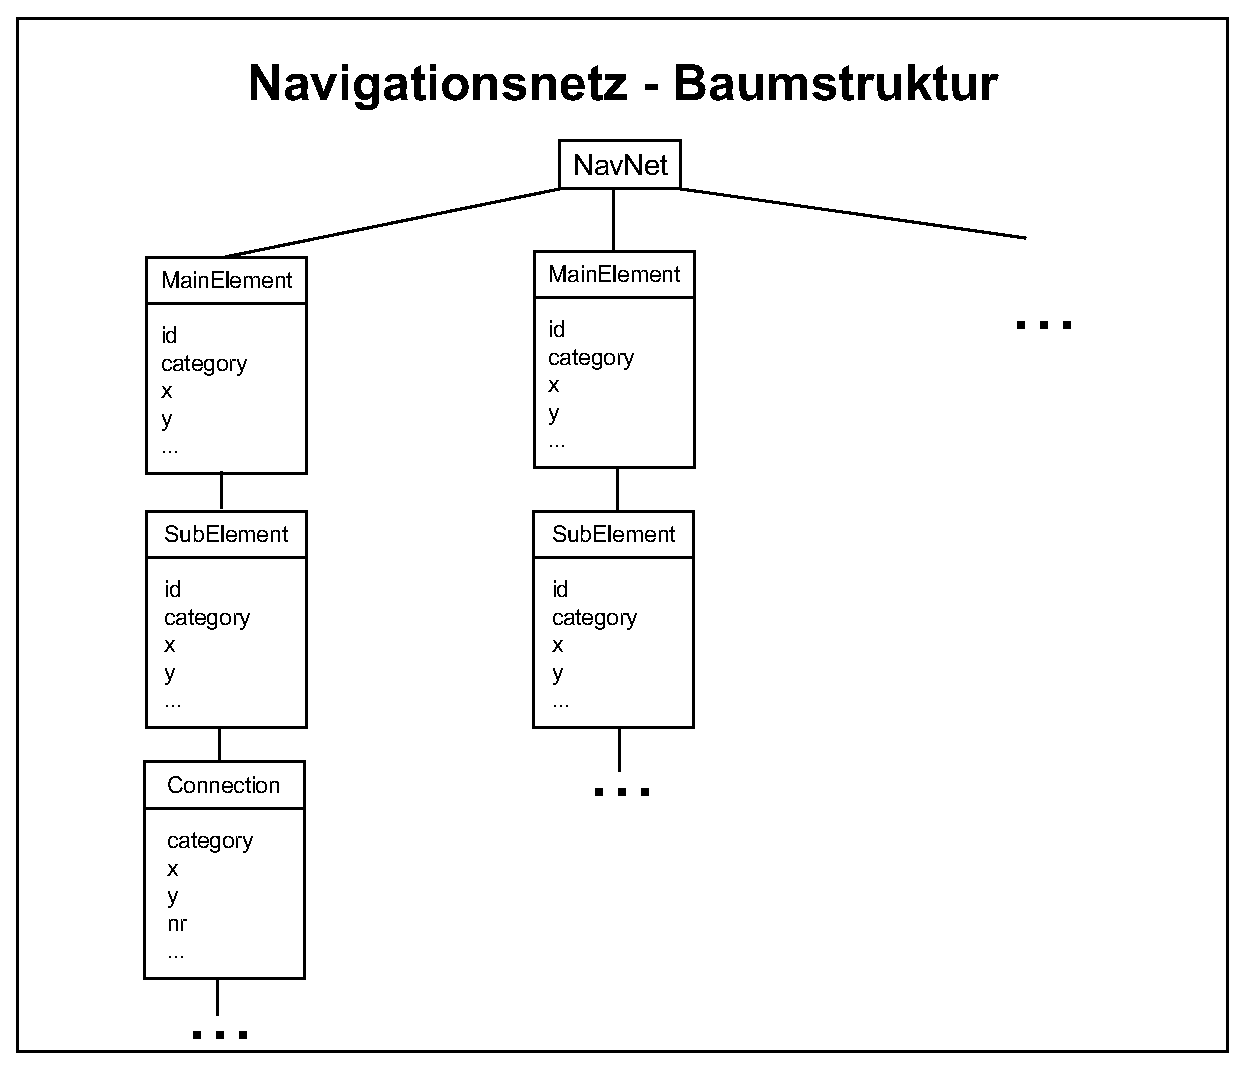
\includegraphics[width=10cm]{figs/baumstruktur}
    \captionbelow{Baumstruktur}
    \label{FIG:baumstruktur}
\end{figure}

\begin{figure}[htbp]
    \centering%
%   \setcapwidth[c]{12cm}%
    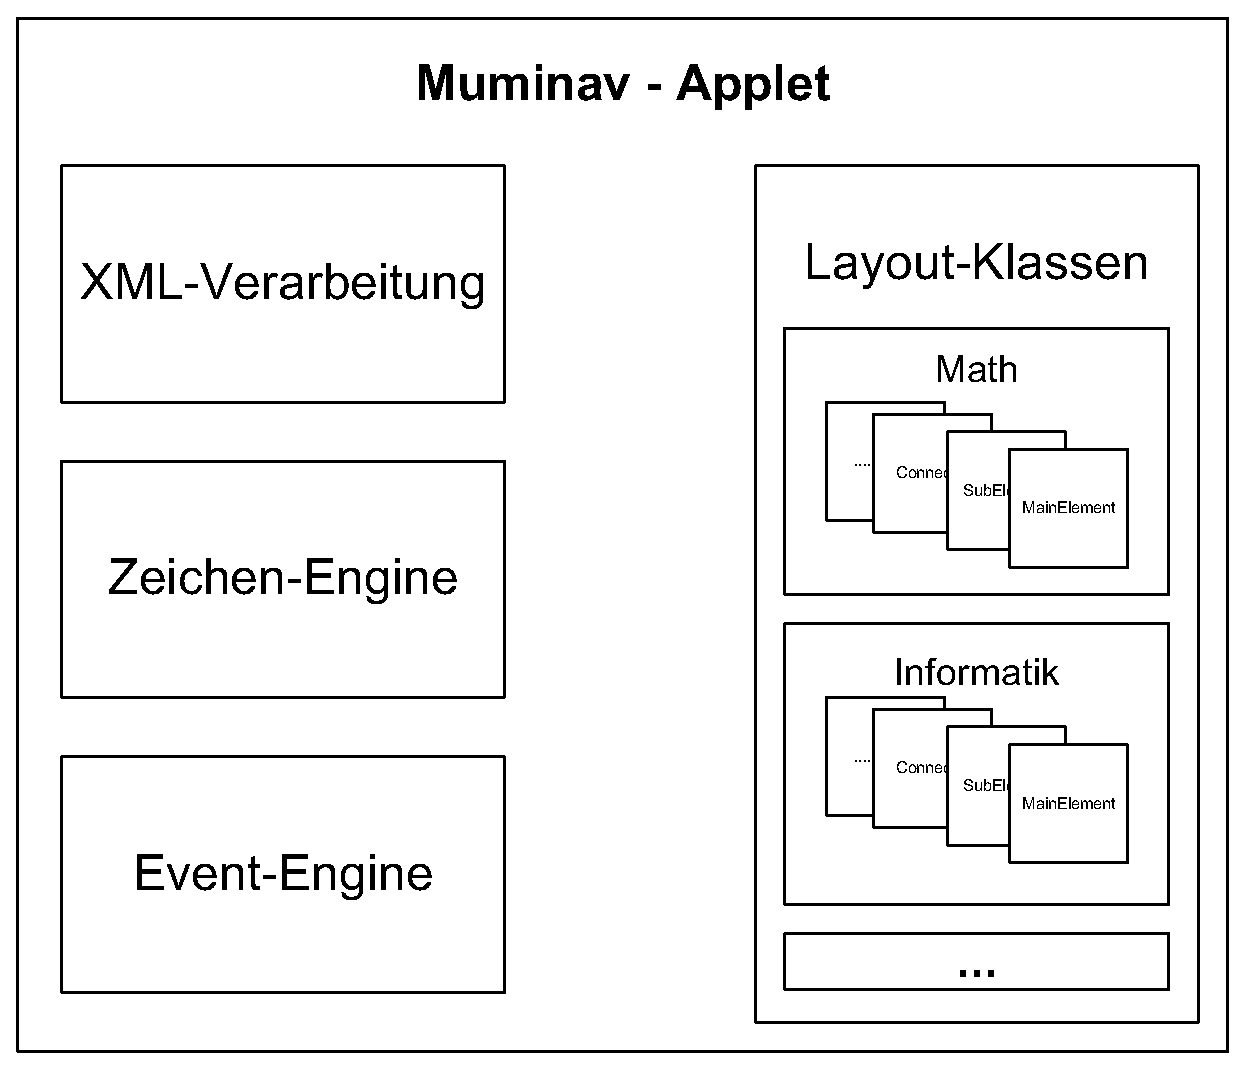
\includegraphics[width=10cm]{figs/aufbau}
    \captionbelow{Aufbau: Haupteile von Muminav}
    \label{FIG:aufbau}
\end{figure}
